\documentclass[12pt,letterpaper]{article}
\usepackage{graphicx,textcomp}
\usepackage{natbib}
\usepackage{setspace}
\usepackage{fullpage}
\usepackage{color}
\usepackage[reqno]{amsmath}
\usepackage{amsthm}
\usepackage{fancyvrb}
\usepackage{amssymb,enumerate}
\usepackage[all]{xy}
\usepackage{endnotes}
\usepackage{lscape}
\newtheorem{com}{Comment}
\usepackage{float}
\usepackage{hyperref}
\newtheorem{lem} {Lemma}
\newtheorem{prop}{Proposition}
\newtheorem{thm}{Theorem}
\newtheorem{defn}{Definition}
\newtheorem{cor}{Corollary}
\newtheorem{obs}{Observation}
\usepackage[compact]{titlesec}
\usepackage{dcolumn}
\usepackage{tikz}
\usetikzlibrary{arrows}
\usepackage{multirow}
\usepackage{xcolor}
\newcolumntype{.}{D{.}{.}{-1}}
\newcolumntype{d}[1]{D{.}{.}{#1}}
\definecolor{light-gray}{gray}{0.65}
\usepackage{url}
\usepackage{listings}
\usepackage{color}

\definecolor{codegreen}{rgb}{0,0.6,0}
\definecolor{codegray}{rgb}{0.5,0.5,0.5}
\definecolor{codepurple}{rgb}{0.58,0,0.82}
\definecolor{backcolour}{rgb}{0.95,0.95,0.92}

\lstdefinestyle{mystyle}{
	backgroundcolor=\color{backcolour},   
	commentstyle=\color{codegreen},
	keywordstyle=\color{magenta},
	numberstyle=\tiny\color{codegray},
	stringstyle=\color{codepurple},
	basicstyle=\footnotesize,
	breakatwhitespace=false,         
	breaklines=true,                 
	captionpos=b,                    
	keepspaces=true,                 
	numbers=left,                    
	numbersep=5pt,                  
	showspaces=false,                
	showstringspaces=false,
	showtabs=false,                  
	tabsize=2
}
\lstset{style=mystyle}
\newcommand{\Sref}[1]{Section~\ref{#1}}
\newtheorem{hyp}{Hypothesis}

\title{Problem Set 1}
\date{Due: September 30, 2024}
\author{Applied Stats/Quant Methods 1}

\begin{document}
	\maketitle
	
	\section*{Instructions}
	\begin{itemize}
	\item Please show your work! You may lose points by simply writing in the answer. If the problem requires you to execute commands in \texttt{R}, please include the code you used to get your answers. Please also include the \texttt{.R} file that contains your code. If you are not sure if work needs to be shown for a particular problem, please ask.
\item Your homework should be submitted electronically on GitHub.
\item This problem set is due before 23:59 on Monday September 30, 2024. No late assignments will be accepted.
%\item Total available points for this homework is 80.
	\end{itemize}
	
	\vspace{1cm}
	\section*{Question 1: Education}

A school counselor was curious about the average of IQ of the students in her school and took a random sample of 25 students' IQ scores. The following is the data set:\\
\vspace{.5cm}

\lstinputlisting[language=R, firstline=36, lastline=36]{my_answers_RJ.C.R}  

\vspace{1cm}

\begin{enumerate}
	\item Find a 90\% confidence interval for the average student IQ in the school.\\
	\lstinputlisting[language=R, firstline=47, lastline=54]{my_answersRJ.C.R}
	
	\item Next, the school counselor was curious  whether  the average student IQ in her school is higher than the average IQ score (100) among all the schools in the country.\\ 
	\noindent Using the same sample, conduct the appropriate hypothesis test with $\alpha=0.05$.

	\lstinputlisting[language=R, firstline=55, lastline=76]{my_answersRJ.C.R}  
\end{enumerate}

\newpage

	\section*{Question 2: Political Economy}

\noindent Researchers are curious about what affects the amount of money communities spend on addressing homelessness. The following variables constitute our data set about social welfare expenditures in the USA. \\
\vspace{.5cm}


\begin{tabular}{r|l}
	\texttt{State} &\emph{50 states in US} \\
	\texttt{Y} & \emph{per capita expenditure on shelters/housing assistance in state}\\
	\texttt{X1} &\emph{per capita personal income in state} \\
	\texttt{X2} &  \emph{Number of residents per 100,000 that are "financially insecure" in state}\\
	\texttt{X3} &  \emph{Number of people per thousand residing in urban areas in state} \\
	\texttt{Region} &  \emph{1=Northeast, 2= North Central, 3= South, 4=West} \\
\end{tabular}

\vspace{.5cm}
\noindent Explore the \texttt{expenditure} data set and import data into \texttt{R}.
\vspace{.5cm}
\lstinputlisting[language=R, firstline=54, lastline=54]{my_answers_RJ.C.R}  
\vspace{.5cm}
\begin{itemize}

\item
Please plot the relationships among \emph{Y}, \emph{X1}, \emph{X2}, and \emph{X3}? What are the correlations among them (you just need to describe the graph and the relationships among them)?

\lstinputlisting[language=R, firstline=116, lastline=116]{my_answersRJ.C.R}
    \begin{enumerate}
	\item[]
	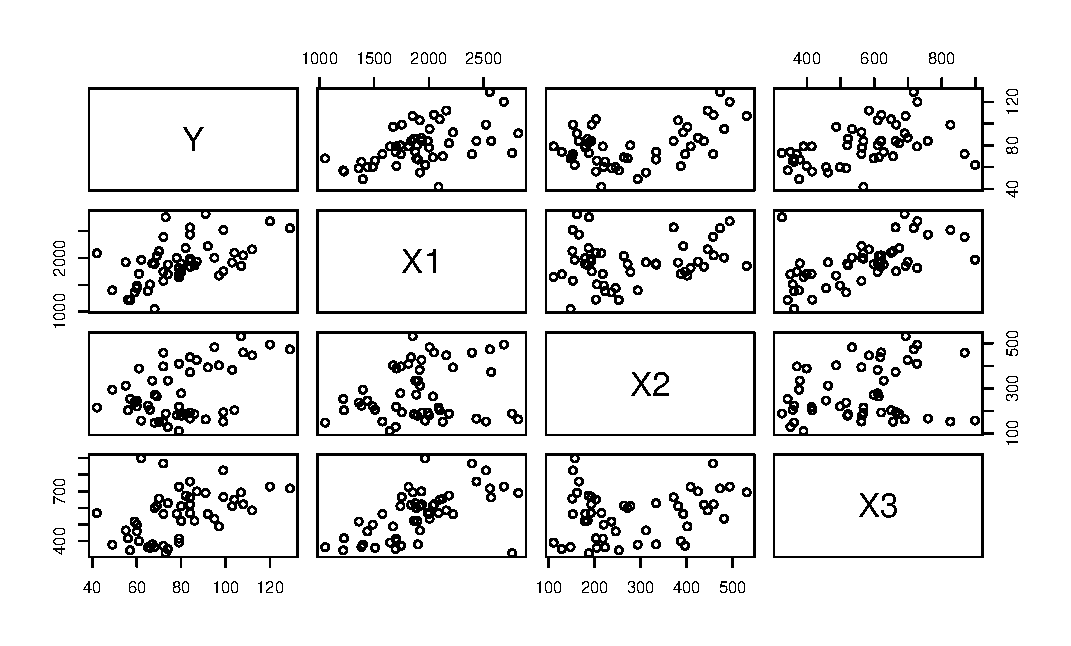
\includegraphics[width=.85\textwidth]{plot.all relationship_RJ.C.pdf}
   \end{enumerate}
   \begin{verbatim}
   	Y is positively correlated with X1, X2, X3
   	X1 is negatively correlated with X2
   	X1 is positively correlated with X3
   	The relationship between X2 and X3 is weak
   \end{verbatim}
\lstinputlisting[language=R, firstline=119, lastline=119]{my_answersRJ.C.R}
	\begin{verbatim}
	  STATE                 Y                X1             X2              X3       
	Length:50          Min.   : 42.00   Min.   :1053   Min.   :111.0   Min.   :326.0  
	Class :character   1st Qu.: 67.25   1st Qu.:1698   1st Qu.:187.2   1st Qu.:426.2  
	Mode  :character   Median : 79.00   Median :1897   Median :241.5   Median :568.0  
	                   Mean   : 79.54   Mean   :1912   Mean   :281.8   Mean   :561.7  
	                   3rd Qu.: 90.00   3rd Qu.:2096   3rd Qu.:391.8   3rd Qu.:661.2  
	                   Max.   :129.00   Max.   :2817   Max.   :531.0   Max.   :899.0 
  \end{verbatim} 
\vspace{.5cm}
\item
Please plot the relationship between \emph{Y} and \emph{Region}? On average, which region has the highest per capita expenditure on housing assistance?

\lstinputlisting[language=R, firstline=133, lastline=135]{my_answersRJ.C.R}
   \begin{enumerate}
   	\item[]
  	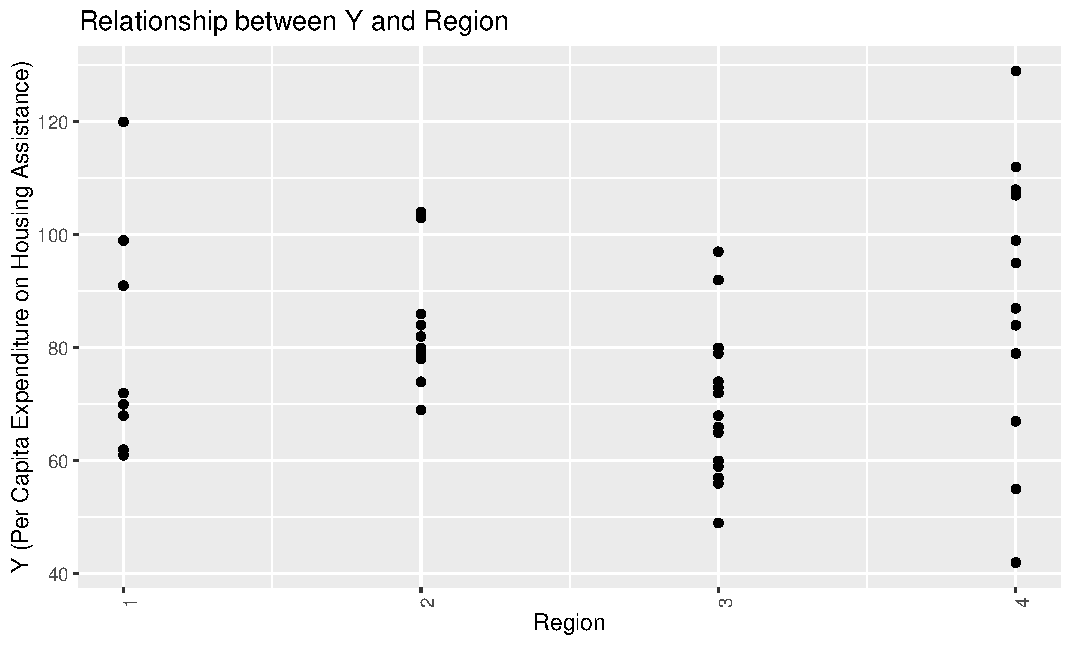
\includegraphics[width=.85\textwidth]{plot.Y.Region_RJ.C.pdf}
   \end{enumerate}
\lstinputlisting[language=R, firstline=137, lastline=138]{my_answersRJ.C.R}
    \begin{verbatim}
    	                  Region        Y
    	                    4        88.30769
    \end{verbatim} 
\vspace{.5cm}
\item
Please plot the relationship between \emph{Y} and \emph{X1}? Describe this graph and the relationship. Reproduce the above graph including one more variable \emph{Region} and display different regions with different types of symbols and colors.

\lstinputlisting[language=R, firstline=145, lastline=147]{my_answersRJ.C.R}
           \begin{enumerate}
           	\item[]
         	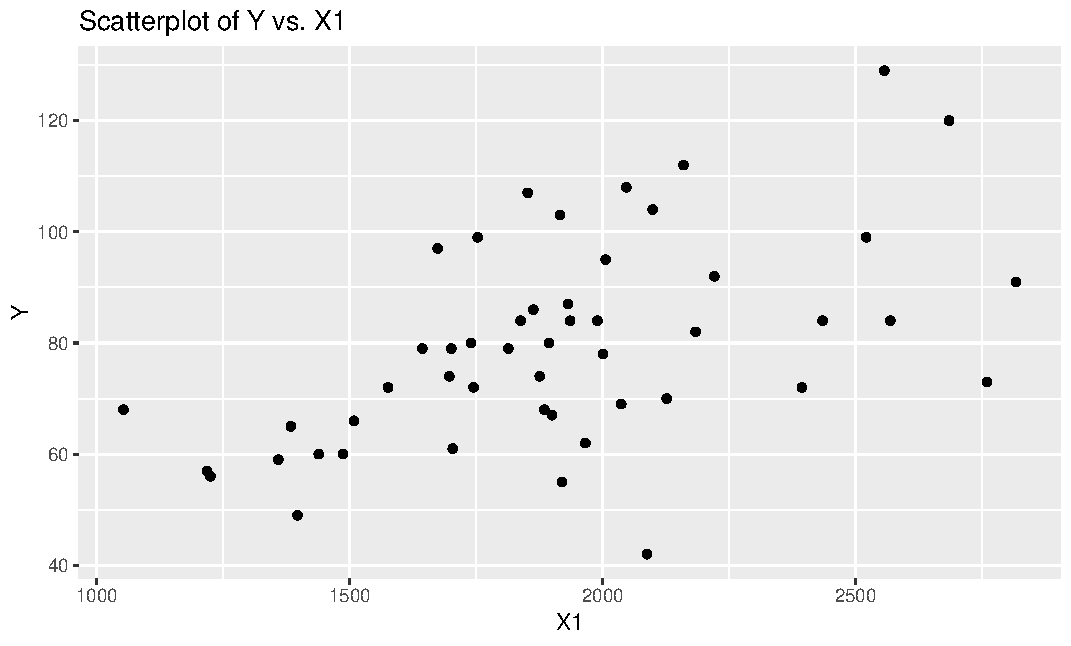
\includegraphics[width=.85\textwidth]{plot.Y.X1_RJ.C.pdf}
           \end{enumerate} 
\lstinputlisting[language=R, firstline=155, lastline=155]{my_answersRJ.C.R}
       %  \begin{table}[htbp]
       %  	\centering
       %  	
===============================================
                        Dependent variable:    
                    ---------------------------
                                 Y             
-----------------------------------------------
X1                           0.025***          
                              (0.006)          
                                               
Constant                     32.546***         
                             (11.034)          
                                               
-----------------------------------------------
Observations                    50             
R2                             0.283           
Adjusted R2                    0.268           
Residual Std. Error      15.836 (df = 48)      
F Statistic           18.920*** (df = 1; 48)   
===============================================
Note:               *p<0.1; **p<0.05; ***p<0.01

       %  \end{table}
       %  problem:The format in the file is correct, but when imported into LaTeX, the format changes
       \begin{table}[!htbp] \centering 
       	\caption{} 
       	\label{} 
       	\begin{tabular}{@{\extracolsep{5pt}}lc} 
       		\\[-1.8ex]\hline 
       		\hline \\[-1.8ex] 
       		& \multicolumn{1}{c}{\textit{Dependent variable:}} \\ 
       		\cline{2-2} 
       		\\[-1.8ex] & Y \\ 
       		\hline \\[-1.8ex] 
       		X1 & 0.025$^{***}$ \\ 
       		& (0.006) \\ 
       		& \\ 
       		Constant & 32.546$^{***}$ \\ 
       		& (11.034) \\ 
       		& \\ 
       		\hline \\[-1.8ex] 
       		Observations & 50 \\ 
       		R$^{2}$ & 0.283 \\ 
       		Adjusted R$^{2}$ & 0.268 \\ 
       		Residual Std. Error & 15.836 (df = 48) \\ 
       		F Statistic & 18.920$^{***}$ (df = 1; 48) \\ 
       		\hline 
       		\hline \\[-1.8ex] 
       		\textit{Note:}  & \multicolumn{1}{r}{$^{*}$p$<$0.1; $^{**}$p$<$0.05; $^{***}$p$<$0.01} \\ 
       	\end{tabular} 
       	 \begin{verbatim}
      	Y is strongly positively correlated with X1
    	as per capita income increases 
    	per capita housing expenditure will also increase
       	\end{verbatim}
       \end{table}  
\lstinputlisting[language=R, firstline=165, lastline=167]{my_answersRJ.C.R}
           \begin{enumerate}
         	\item[]
        	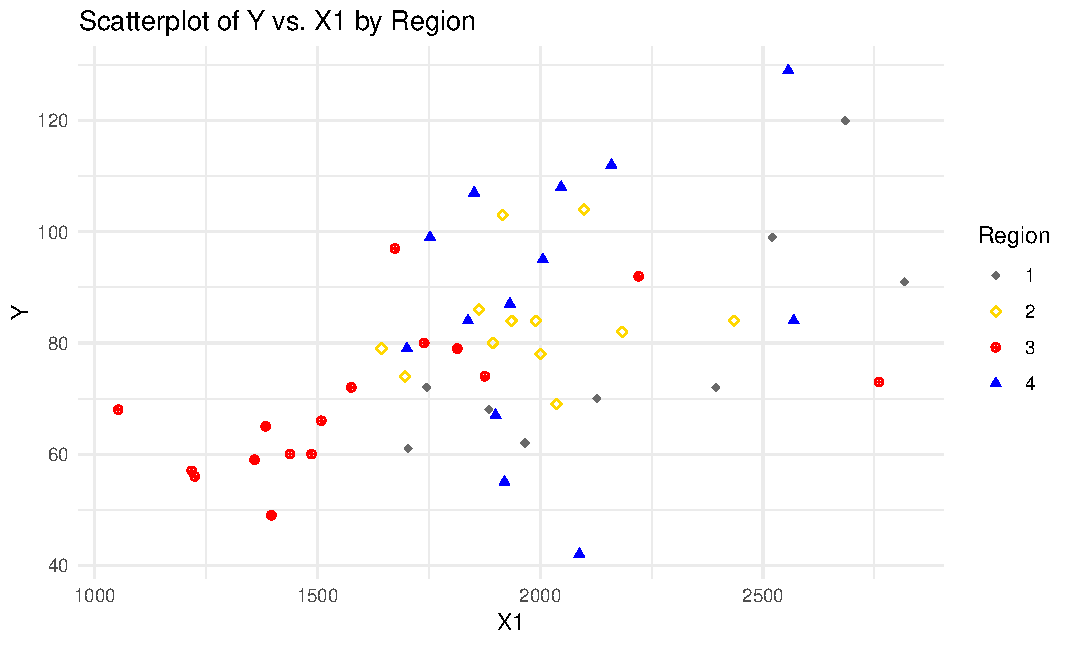
\includegraphics[width=.85\textwidth]{plot.symbols.colors_RJ.C.pdf}
           \end{enumerate} 
               % Complete the question about Y/X1
\lstinputlisting[language=R, firstline=174, lastline=176]{my_answersRJ.C.R}
        \begin{enumerate}
    	 \item[]
	     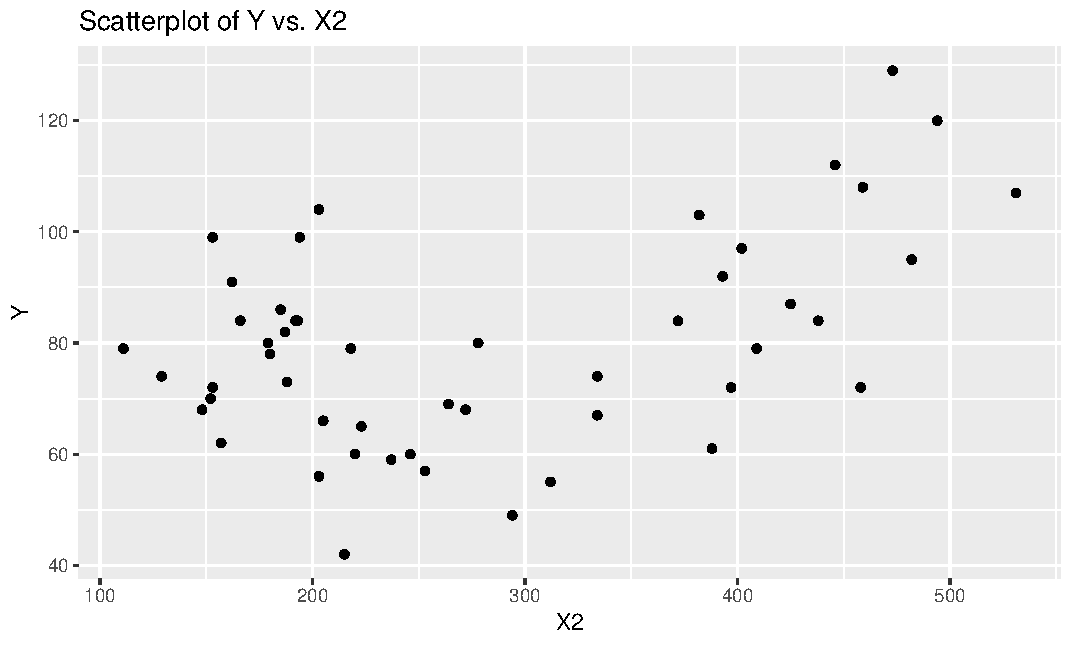
\includegraphics[width=.85\textwidth]{plot.Y.X2_RJ.C.pdf}
        \end{enumerate}
\lstinputlisting[language=R, firstline=185, lastline=185]{my_answersRJ.C.R}
       \begin{table}[!htbp] \centering 
	    \caption{} 
	    \label{} 
   	    \begin{tabular}{@{\extracolsep{5pt}}lc} 
		    \\[-1.5ex]\hline 
		    \hline \\[-1.5ex] 
		    & \multicolumn{1}{c}{\textit{Dependent variable:}} \\ 
		    \cline{2-2} 
		    \\[-1.5ex] & Y \\ 
		    \hline \\[-1.5ex] 
		    X2 & 0.070$^{***}$ \\ 
		    & (0.020) \\ 
		    & \\ 
		    Constant & 57.761$^{***}$ \\ 
		    & (6.164) \\ 
		    & \\ 
		    \hline \\[-1.5ex] 
		    Observations & 50 \\ 
		    R$^{2}$ & 0.201 \\ 
		    Adjusted R$^{2}$ & 0.184 \\ 
		    Residual Std. Error & 16.714 (df = 48) \\ 
		    F Statistic & 12.072$^{***}$ (df = 1; 48) \\ 
		    \hline 
		    \hline \\[-1.5ex] 
		    \textit{Note:}  & \multicolumn{1}{r}{$^{*}$p$<$0.1; $^{**}$p$<$0.05; $^{***}$p$<$0.01} \\ 
	     \end{tabular} 
	     \begin{verbatim}
	     	  Y is moderately positively correlated with X2,
	  	indicating that in continents with unstable economic conditions,
	  	the housing assistance rate is high
	     \end{verbatim}
       \end{table} 
\lstinputlisting[language=R, firstline=195, lastline=197]{my_answersRJ.C.R}
           \begin{enumerate}
   	        \item[]
	        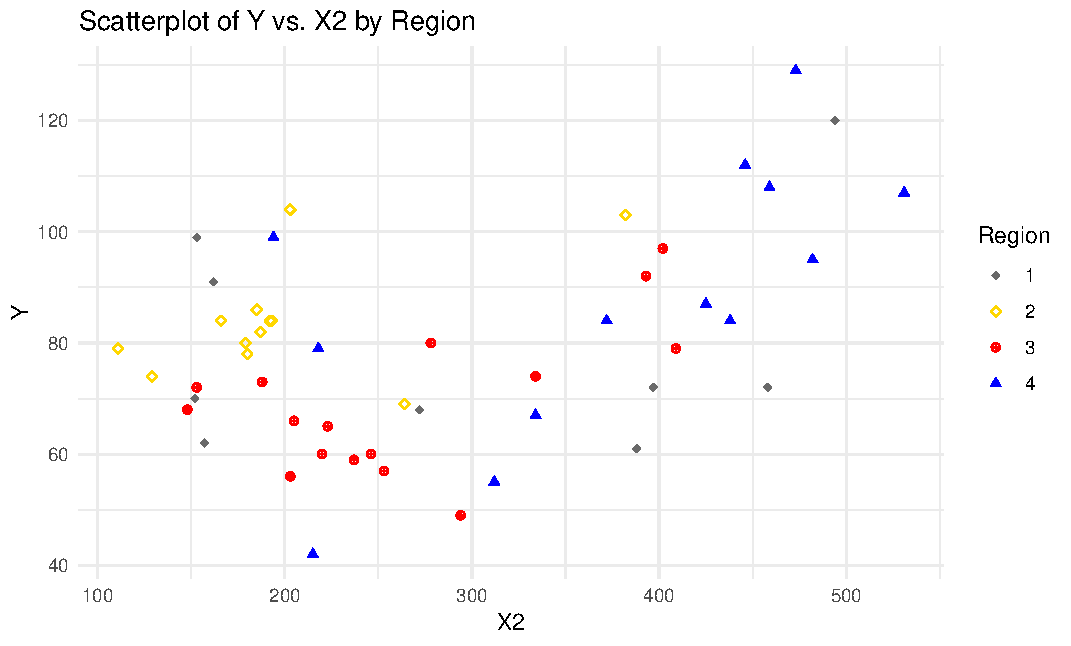
\includegraphics[width=.85\textwidth]{plot.symbols.colors2_RJ.C.pdf}
           \end{enumerate}
            % Complete the question about Y/X2
\lstinputlisting[language=R, firstline=204, lastline=206]{my_answersRJ.C.R}
          \begin{enumerate}
	       \item[]
	       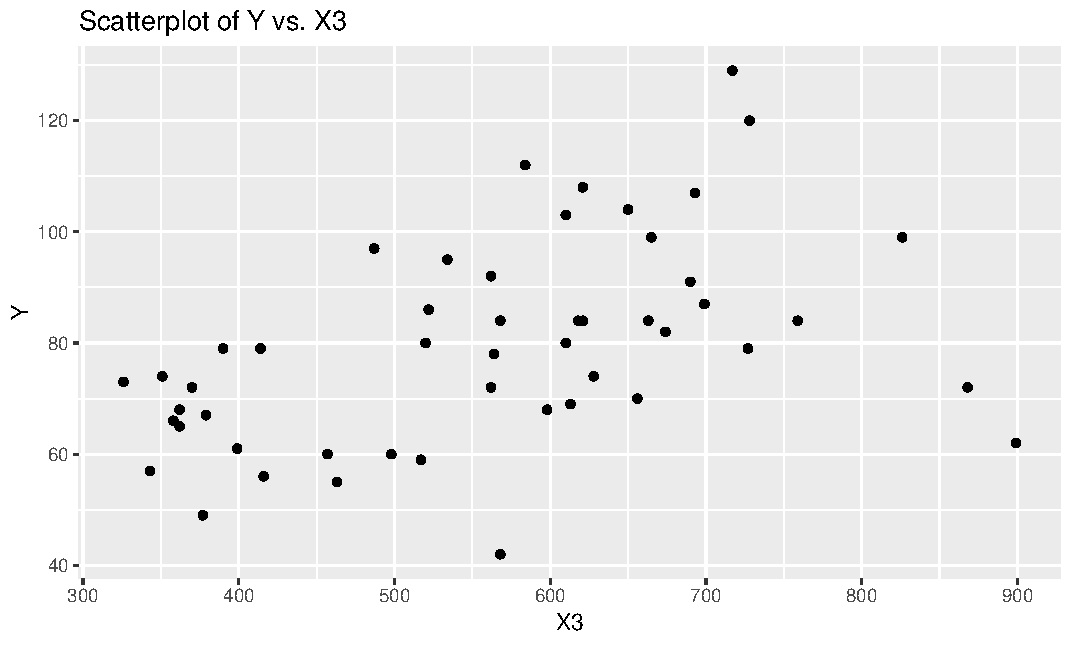
\includegraphics[width=.85\textwidth]{plot.Y.X3_RJ.C.pdf}
          \end{enumerate}
\lstinputlisting[language=R, firstline=185, lastline=185]{my_answersRJ.C.R}
  \begin{table}[!htbp] \centering 
	\caption{} 
	\label{} 
	\begin{tabular}{@{\extracolsep{5pt}}lc} 
		\\[-1.8ex]\hline 
		\hline \\[-1.8ex] 
		& \multicolumn{1}{c}{\textit{Dependent variable:}} \\ 
		\cline{2-2} 
		\\[-1.8ex] & Y \\ 
		\hline \\[-1.8ex] 
		X3 & 0.059$^{***}$ \\ 
		& (0.016) \\ 
		& \\ 
		Constant & 43.306$^{***}$ \\ 
		& (9.461) \\ 
		& \\ 
		\hline \\[-1.8ex] 
		Observations & 50 \\ 
		R$^{2}$ & 0.215 \\ 
		Adjusted R$^{2}$ & 0.199 \\ 
		Residual Std. Error & 16.567 (df = 48) \\ 
		F Statistic & 13.1146$^{***}$ (df = 1; 48) \\ 
		\hline 
		\hline \\[-1.8ex] 
		\textit{Note:}  & \multicolumn{1}{r}{$^{*}$p$<$0.1; $^{**}$p$<$0.05; $^{***}$p$<$0.01} \\ 
	\end{tabular}
	 \begin{verbatim} 
   	Y is moderately positively correlated with X3
	in areas with higher levels of urbanization
	there is more expenditure on housing assistance
	 \end{verbatim}
  \end{table} 
\lstinputlisting[language=R, firstline=225, lastline=227]{my_answersRJ.C.R}
    \begin{enumerate}
	  \item[]
	  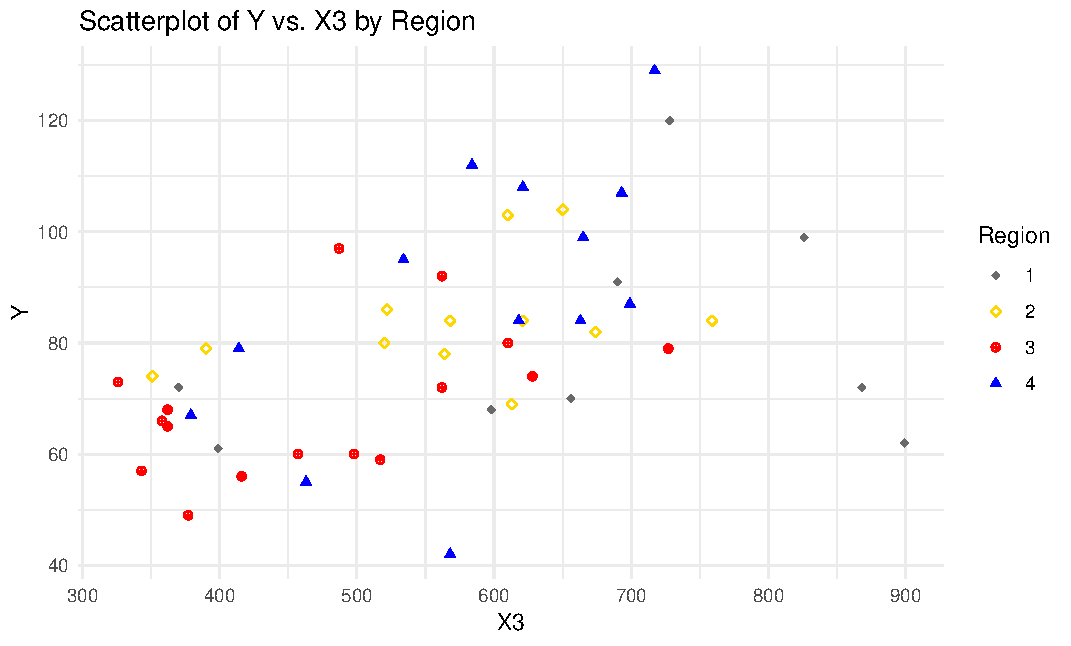
\includegraphics[width=.85\textwidth]{plot.symbols.colors3_RJ.C.pdf}
    \end{enumerate}
               % Complete the question about Y/X3

\lstinputlisting[language=R, firstline=234, lastline=236]{my_answersRJ.C.R}
    \begin{enumerate}
  	  \item[]
	  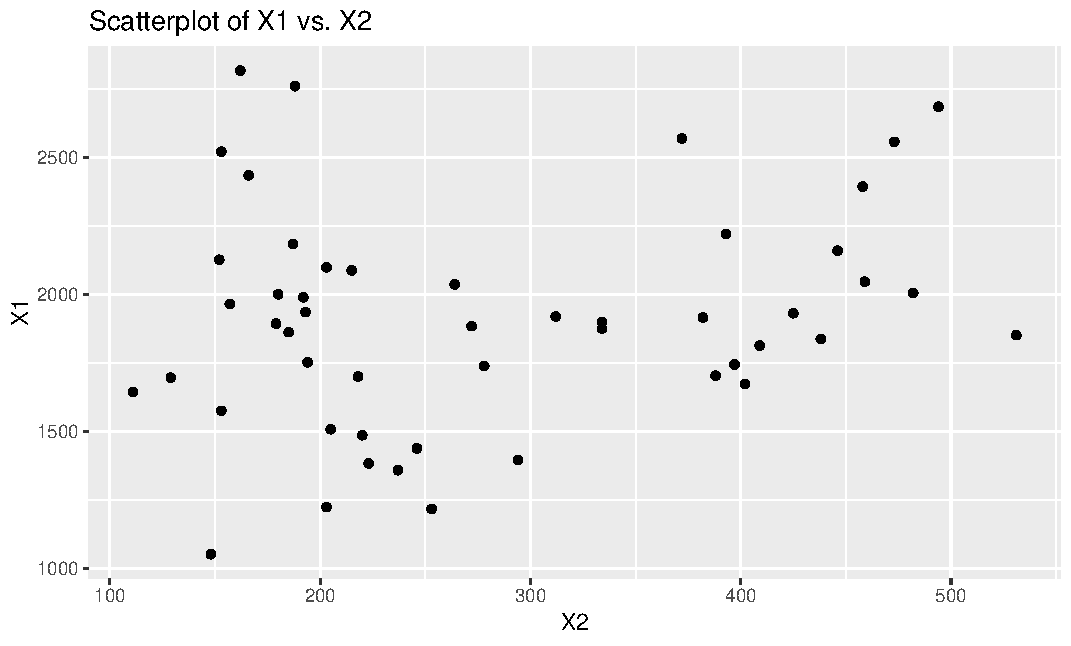
\includegraphics[width=.85\textwidth]{plot.X1.X2_RJ.C.pdf}
    \end{enumerate}
\lstinputlisting[language=R, firstline=245, lastline=245]{my_answersRJ.C.R}
  \begin{table}[!htbp] \centering 
	\caption{} 
	\label{} 
	\begin{tabular}{@{\extracolsep{5pt}}lc} 
		\\[-1.8ex]\hline 
		\hline \\[-1.8ex] 
		& \multicolumn{1}{c}{\textit{Dependent variable:}} \\ 
		\cline{2-2} 
		\\[-1.8ex] & X1 \\ 
		\hline \\[-1.8ex] 
		X2 & 0.696$^{***}$ \\ 
		& (0.478) \\ 
		& \\ 
		Constant & 1715.655$^{***}$ \\ 
		& (145.981) \\ 
		& \\ 
		\hline \\[-1.8ex] 
		Observations & 50 \\ 
		R$^{2}$ & 0.042 \\ 
		Adjusted R$^{2}$ & 0.022 \\ 
		Residual Std. Error & 395.854 (df = 48) \\ 
		F Statistic & 2.119$^{***}$ (df = 1; 48) \\ 
		\hline 
		\hline \\[-1.8ex] 
		\textit{Note:}  & \multicolumn{1}{r}{$^{*}$p$<$0.1; $^{**}$p$<$0.05; $^{***}$p$<$0.01} \\ 
	\end{tabular} 
	 \begin{verbatim} 
		X1 is negatively correlated with X2,
		indicating that areas with high per capita income 
		have fewer economically unstable residents
	\end{verbatim}
  \end{table} 
  
\lstinputlisting[language=R, firstline=255, lastline=257]{my_answersRJ.C.R}
  \begin{enumerate}
	\item[]
	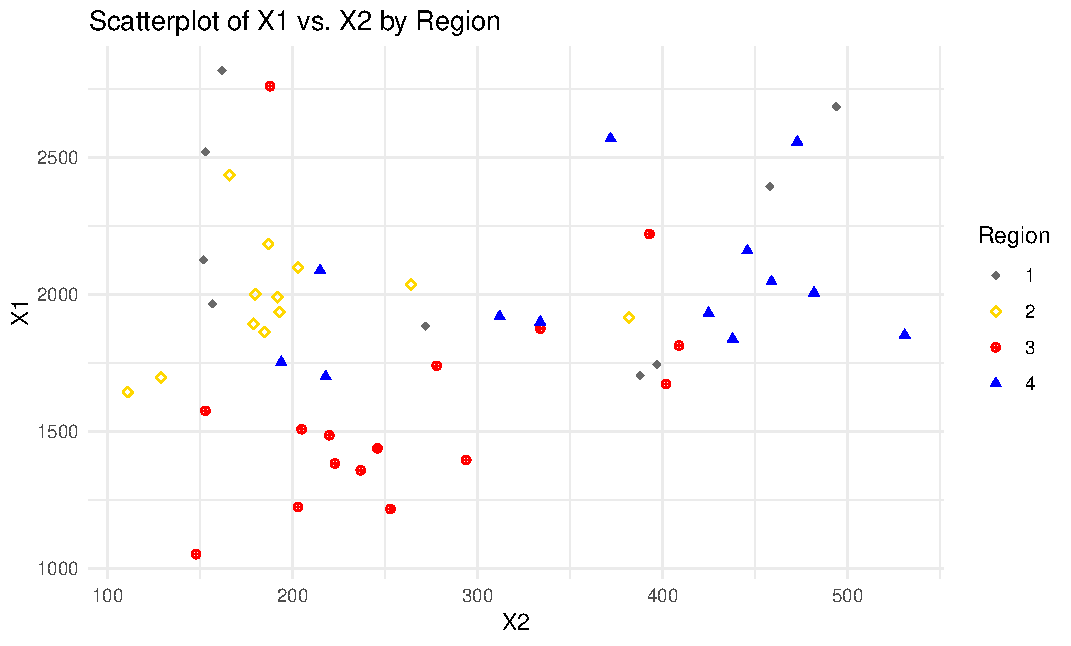
\includegraphics[width=.85\textwidth]{plot.symbols.colors4_RJ.C.pdf}
  \end{enumerate}
                  % Complete the question about X1/X2

\lstinputlisting[language=R, firstline=264, lastline=266]{my_answersRJ.C.R}
  \begin{enumerate}
	\item[]
	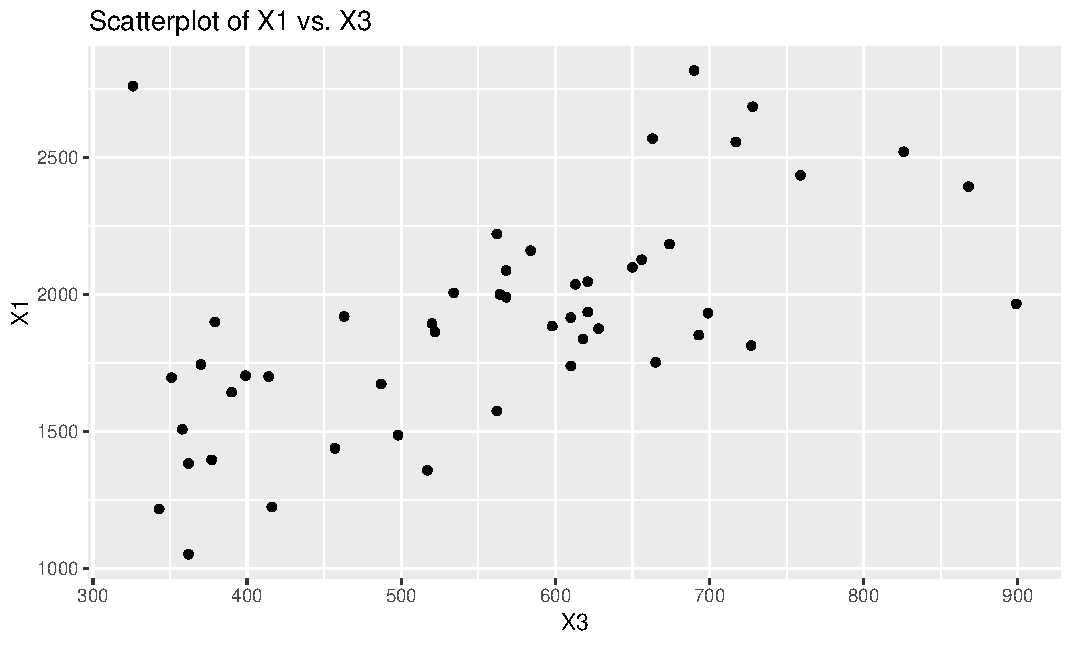
\includegraphics[width=.85\textwidth]{plot.X1.X3_RJ.C.pdf}
  \end{enumerate}
\lstinputlisting[language=R, firstline=275, lastline=275]{my_answersRJ.C.R}
  \begin{table}[!htbp] \centering 
	\caption{} 
	\label{} 
	\begin{tabular}{@{\extracolsep{5pt}}lc} 
		\\[-1.8ex]\hline 
		\hline \\[-1.8ex] 
		& \multicolumn{1}{c}{\textit{Dependent variable:}} \\ 
		\cline{2-2} 
		\\[-1.8ex] & X1 \\ 
		\hline \\[-1.8ex] 
		X3 & 1.643$^{***}$ \\ 
		& (0.320) \\ 
		& \\ 
		Constant & 988.947$^{***}$ \\ 
		& (185.614) \\ 
		& \\ 
		\hline \\[-1.8ex] 
		Observations & 50 \\ 
		R$^{2}$ & 0.354 \\ 
		Adjusted R$^{2}$ & 0.341 \\ 
		Residual Std. Error & 325.029 (df = 48) \\ 
		F Statistic & 26.341$^{***}$ (df = 1; 48) \\ 
		\hline 
		\hline \\[-1.8ex] 
		\textit{Note:}  & \multicolumn{1}{r}{$^{*}$p$<$0.1; $^{**}$p$<$0.05; $^{***}$p$<$0.01} \\ 
	\end{tabular} 
	\begin{verbatim} 
		X1 is positively correlated with X3,
		indicating that areas with high urbanization
		 have higher per capita income
	\end{verbatim}
  \end{table} 
\lstinputlisting[language=R, firstline=285, lastline=287]{my_answersRJ.C.R}
  \begin{enumerate}
	\item[]
	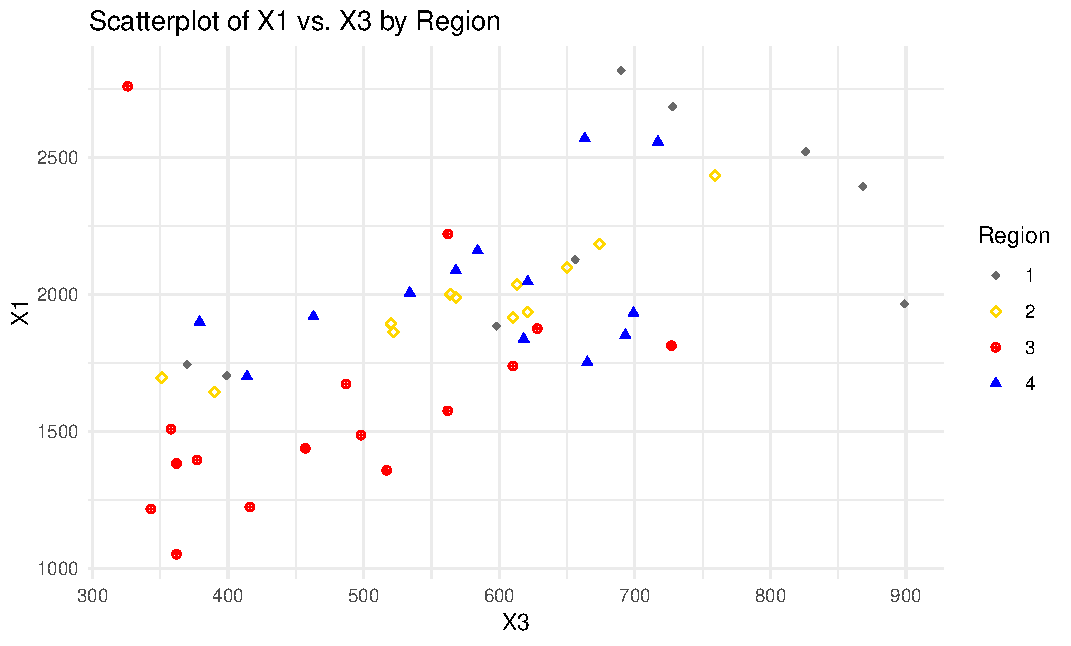
\includegraphics[width=.85\textwidth]{plot.symbols.colors5_RJ.C.pdf}
  \end{enumerate}
                % Complete the question about X1/X3
                
\lstinputlisting[language=R, firstline=294, lastline=296]{my_answersRJ.C.R}
  \begin{enumerate}
	\item[]
	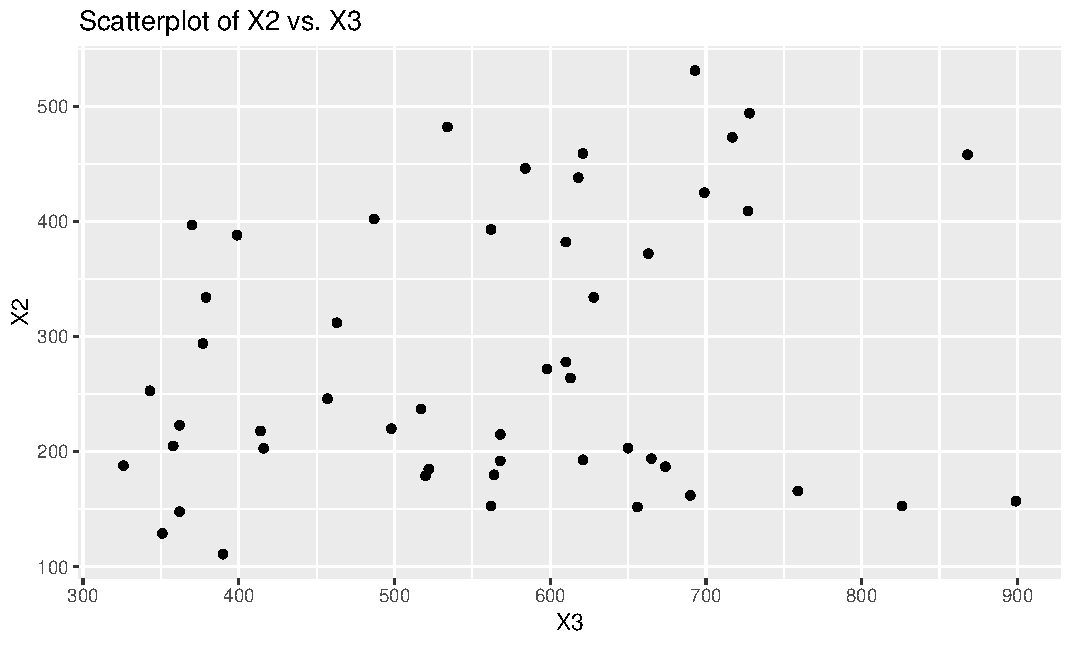
\includegraphics[width=.85\textwidth]{plot.X2.X3_RJ.C.pdf}
  \end{enumerate}
\lstinputlisting[language=R, firstline=305, lastline=305]{my_answersRJ.C.R}
  \begin{table}[!htbp] \centering 
	\caption{} 
	\label{} 
	\begin{tabular}{@{\extracolsep{5pt}}lc} 
		\\[-1.8ex]\hline 
		\hline \\[-1.8ex] 
		& \multicolumn{1}{c}{\textit{Dependent variable:}} \\ 
		\cline{2-2} 
		\\[-1.8ex] & X2 \\ 
		\hline \\[-1.8ex] 
		X3 & 0.180$^{***}$ \\ 
		& (0.115) \\ 
		& \\ 
		Constant & 180.609$^{***}$ \\ 
		& (66.509) \\ 
		& \\ 
		\hline \\[-1.8ex] 
		Observations & 50 \\ 
		R$^{2}$ & 0.049 \\ 
		Adjusted R$^{2}$ & 0.029 \\ 
		Residual Std. Error & 116.465 (df = 48) \\ 
		F Statistic & 2.465$^{***}$ (df = 1; 48) \\ 
		\hline 
		\hline \\[-1.8ex] 
		\textit{Note:}  & \multicolumn{1}{r}{$^{*}$p$<$0.1; $^{**}$p$<$0.05; $^{***}$p$<$0.01} \\ 
	\end{tabular} 
	\begin{verbatim} 
	The correlation between X2 and X3 is weak
	the degree of urbanization has little to do with economic instability
	\end{verbatim}
  \end{table}
\lstinputlisting[language=R, firstline=315, lastline=317]{my_answersRJ.C.R}
  \begin{enumerate}
	\item[]
	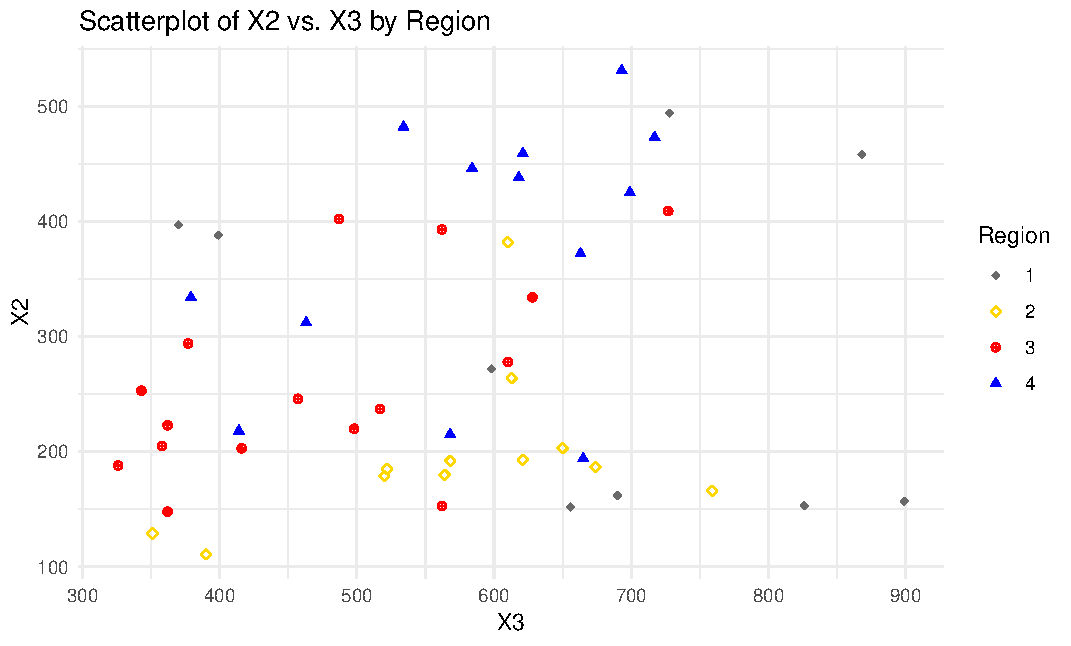
\includegraphics[width=.85\textwidth]{plot.symbols.colors6_RJ.C.pdf}
  \end{enumerate}
               % Complete the question about X2/X3

\end{itemize}


\end{document}
